\section{Part A: Soling Geodesics}
\label{Sec2}

Using the python library \code{sympy}\footnote{This does not come directly by installing python using the \code{pip} command. To install it, simply type, \code{pip install --user sympy}.}, we evaluate the Christoffel symbols \eqref{Christoffel} and then use them to construct the force functions on the right-hand side of \eqref{EOM} for the coordinate velocities by also inputting the additional $D$-acceleration $a^{\mu}$.

We have implemented different integration schemes seen in class. Namely, we have implemented Forward Euler, RK2, RK4, Leapfrog and Verlet as well as the adaptive step size versions for the explicit integrators.
%The five integration schemes have the following difference equations,
% WRITE DIFFERENCE EQUATIONS FOR 5 INTEGRATORS

The inputs and outputs of the program are as the following tables \ref{tbl:INPUT} and \ref{tbl:OUTPUT} indicate respectively,
\begin{table}[H]
	\centering
	\begin{tabular}{|c|c|}
		\hline
		Input Parameters & Description \\
		\hline
		\hline
		$x^{\mu}$ & Coordinate system to be used \\
		\hline
		$g_{\mu\nu}(x)$ & Metric tensor components in the $\{x^{\mu}\}$-coordinate system \\
		\hline
		$a^{\mu}$ & $D$-acceleration associated with non-gravitational interaction \\
		\hline
		$t_0$ & Initial coordinate time instant \\
		\hline
		$t_{N}$ & Final coordinate time instant \\
		\hline
		$N$ & Number of time steps to be taken \\
		\hline
		$x^{i}_0$, $i=1,\dots,D-1$ & Initial spatial position at coordinate time $t_0$\\
		\hline
		$\upsilon^{i}_0$, $i=1,\dots,D-1$ & Initial coordinate spatial velocity at coordinate time $t_0$\\
		\hline
		INTEGRATOR & Integration scheme to be used \\
		\hline
	\end{tabular}
	\caption{Input parameters}
	\label{tbl:INPUT}
\end{table}

\begin{table}[H]
	\centering
	\begin{tabular}{|c|c|}
		\hline
		Output Parameters & Description \\
		\hline
		\hline
		$x^{i}(t)$, $i=1,\dots,D-1$ & Spatial position at coordinates times $t\in[t_{0},t_{N}]$ \\
		\hline
		$\upsilon^{i}(t)$, $i=1,\dots,D-1$ & Spatial coordinate velocity at coordinate times $t\in[t_{0},t_{N}]$\\
		\hline
		$u_{\mu}(t)$, $i=0,\dots,D-1$ & Covariant $D$-velocity at coordinate times $t\in[t_{0},t_{N}]$\\
		\hline
	\end{tabular}
	\caption{Output parameters}
	\label{tbl:OUTPUT}
\end{table}

From the covariant $D$-velocity, one can also read the energy and angular momentum of the particle around the $x_{D-1}$-axes whose rotations are associated with the azimuthal angle $\phi \equiv \theta_{D-1}$ when using spherical coordinates,
\be\ba
	E &\equiv -mu_{0} \\
	L &\equiv mu_{D-1}
\ea\ee

\subsection{Schwarzschild Metric}
As a first test, we solve the geodesics for motion around a Schwarzschild black hole whose geometry is,
\be\ba
	ds_{S}^2 &= -f_{S}(r)dt^2 + \frac{dr^2}{f_{S}(r)} + r^2d\Omega_{D-2}^2 \\
	f_{S}(r) &= 1-\left(\frac{R_{S}}{r}\right)^{D-3}
\ea\ee
where $R_{S}$ is the Schwarzschild radius related to the mass $M$ of the black hole (ADM mass) according to,
\be
	R_{S}^{D-3} = \frac{16\pi GM}{(D-2)\Omega_{D-2}}
\ee
with $\Omega_{D-2}$ the surface of a unit $(D-1)$-dimensional sphere,
\be
	\Omega_{D-2} = Area(S^{D-2}) = (D-1)\frac{\pi^{\frac{D-1}{2}}}{\Gamma\left(\frac{D+1}{2}\right)}
\ee
and $d\Omega_{D-2}^2$ is the infinitesimal length on $S^{D-2}$,
\be
	d\Omega_{D-2}^{2} = \sum_{n=2}^{D-1}\left(\prod_{m=2}^{n-1}\sin^2\theta_{m}\right)d\theta_{n}^2
\ee
Note that we have indexed the angle variables from $2$ to $D-1$ to remind that the $x^1$ coordinate is $r$.

The Schwarzschild black hole is equipped with an event horizon\footnote{The event horizons are null surfaces. For the case of the event horizons located at the surfaces of constant radial coordinate $r_{H} = const.$, the condition they must obey is $g^{rr}\mid_{r=r_{H}}=0$.} at precisely the Schwarzschild radius,
\be
	r_{H} = R_{S}
\ee
and signifies the limit of no return. Quite remarkably, a stationary observe will never see the massive particle falling inside the black hole; the particle will appear to slow down near the event horizon until it finally freezes at $r=r_{H}$ and disappears due to infinite redshift. This is a property of all black hole solutions.

\subsubsection{Run 1: Bound trajectory}
For the first run, we take $D=4$ and the following initial conditions,
\begin{table}[H]
	\centering
	\begin{tabular}{|c|c|}
		\hline
		$t_0$ & 0.0 \\
		\hline
		$r_0$ & 10.0 \\
		\hline
		$\theta_0$ & $\frac{\pi}{2}$ \\
		\hline
		$\phi_0$ & 0.0 \\
		\hline
		\hline
		$\upsilon_{r0}$ & -0.03 \\
		\hline
		$\upsilon_{\theta0}$ & 0.0 \\
		\hline
		$\upsilon_{\phi0}$ & 0.03 \\
		\hline
	\end{tabular}
	\caption[Run 1: Initial Conditions]{Run 1: Initial Conditions.}
	\label{tbl:RUN1_IC}
\end{table}

These initial conditions ensure a specific energy $\frac{E}{m} = 0.9501784 < 1$ allowing a bound trajectory. Running using the RK4 integrator with $N=10000$ iterations and final time instant $t_{N} = 1000.0$, we output figures \ref{fig:RUN1_xv} and \ref{fig:RUN1_U}.

\begin{figure}
	\centering
	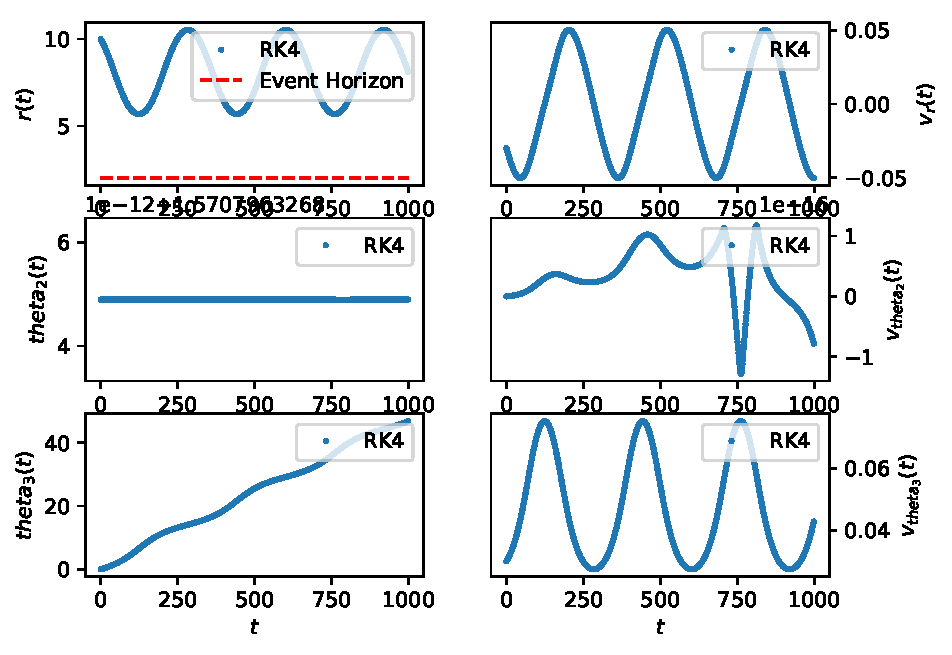
\includegraphics[height=8cm]{Figures/xv_t_Rotating.pdf}
	\caption[Run 1: Coordinate positions and velocities]{Run 1: Coordinate positions and velocities for a bound trajectory in 4-dimensional Schwarzschild solution.}
	\label{fig:RUN1_xv}
\end{figure}

\begin{figure}
	\centering
	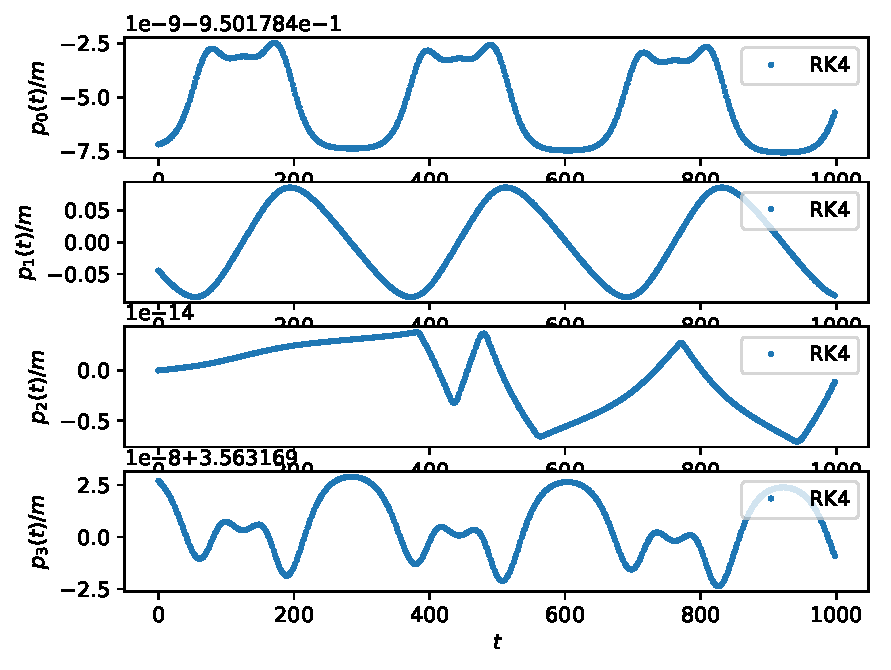
\includegraphics[height=8cm]{Figures/U_t_Rotating.pdf}
	\caption[Run 1: 4-velocity]{Run 1: 4-velocity components for a bound trajectory in 4-dimensional Schwarzschild solution.}
	\label{fig:RUN1_U}
\end{figure}

\subsubsection{Run 2: Doomed trajectory}
For the second run, we take $D=4$ and the following initial conditions,
\begin{table}[H]
	\centering
	\begin{tabular}{|c|c|}
		\hline
		$t_0$ & 0.0 \\
		\hline
		$r_0$ & 3.0 \\
		\hline
		$\theta_0$ & $\frac{\pi}{2}$ \\
		\hline
		$\phi_0$ & 0.0 \\
		\hline
		\hline
		$\upsilon_{r0}$ & -0.3 \\
		\hline
		$\upsilon_{\theta0}$ & 0.0 \\
		\hline
		$\upsilon_{\phi0}$ & 0.0 \\
		\hline
	\end{tabular}
	\caption[Run 2: Initial Conditions]{Run 2: Initial Conditions.}
	\label{tbl:RUN2_IC}
\end{table}

These initial conditions account for an unbound trajectory with a specific energy $\frac{E}{m} = 1.41833 > 1$ but the angular velocity $\upsilon_{\phi0}$ is small enough to not escape the black hole. Running using the RK4 integrator again with $N=300$ steps and final time instant $t_{N} = 10.0$, we output figures \ref{fig:RUN2_xv} and \ref{fig:RUN2_U}.

\begin{figure}
	\centering
	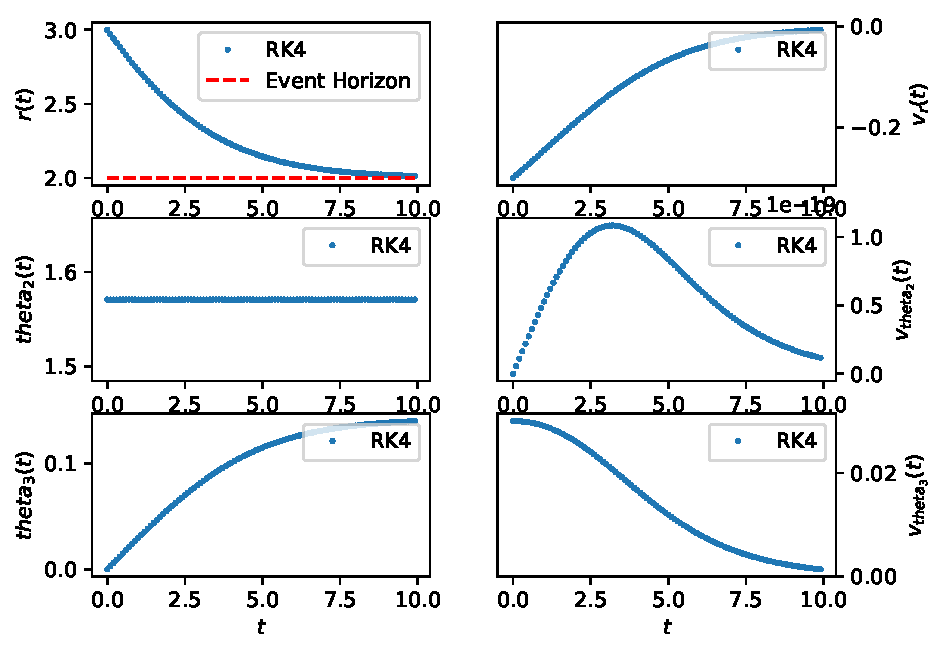
\includegraphics[height=8cm]{Figures/xv_t_Falling.pdf}
	\caption[Run 2: Coordinate positions and velocities]{Run 2: Coordinate positions and velocities for an unbound, doomed trajectory in 4-dimensional Schwarzschild solution.}
	\label{fig:RUN2_xv}
\end{figure}

\begin{figure}
	\centering
	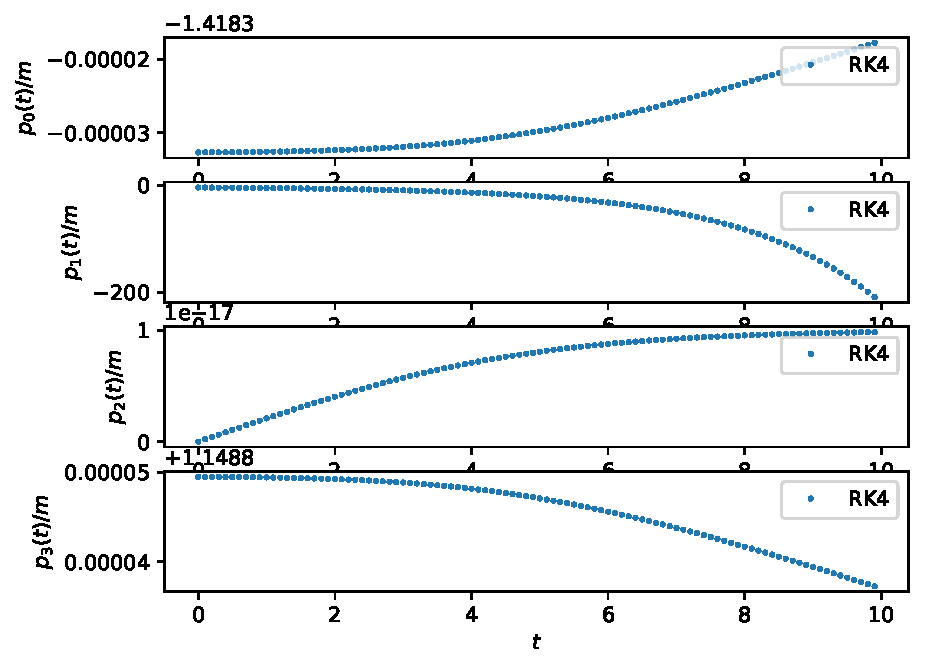
\includegraphics[height=8cm]{Figures/U_t_Falling.pdf}
	\caption[Run 2: 4-velocity]{Run 2: 4-velocity components for a unbound, doomed trajectory in 4-dimensional Schwarzschild solution.}
	\label{fig:RUN2_U}
\end{figure}

\subsection{Reissner-Nordstr\"{o}m Metric}
A second test, would be to run our program for motion around a Reissner-Nordstro\"{o}m black hole,
\be\ba
	ds_{RN}^2 &= -f_{RN}(r)dt^2 + \frac{dr^2}{f_{RN}(r)} + r^2d\Omega_{D-2}^2 \\
	f_{RN}(r) &= 1-\left(\frac{R_{S}}{r}\right)^{D-3} + \left(\frac{A}{r}\right)^{2(D-3)}
\ea\ee
where $A$ is related to the total charge $Q$ of the black hole according to,
\be
	A^{2(D-3)} = \frac{8\pi GQ^2}{(D-2)(D-3)}
\ee

In contrast to the Schwarzschild solution, the Reissner-Nordstr\"{o}m black hole has two event horizons,
\be
	r_{H}^{\pm} = \frac{R_{S}}{2}\left( 1 \pm \sqrt{1 - 4\left(\frac{A}{R_{S}}\right)^{2(D-3)}} \right)^{\frac{1}{D-3}}
\ee
from which, however, only the outer horizon can be formed from physical processes, $r_{H} = r_{H}^{+}$; the inner event horizon is a mathematical artifact.

This run would also test the implementation of additional non-gravitational forces. We leave this analysis for future development.